
% Лабораторная работа по криптографии № 1
% Михедов Константин Константинович

% Тип документа: статья, на бумаге А4
\documentclass[a4paper]{article}

% Подключение сторонних tex файлов 
\usepackage{import}


% Основные данные - ВУЗ, факультет, город...
\import{./../../stuff/tex}{config.tex}
% Небольшой набор инструментов
\import{./../../stuff/tex}{tools.tex}

% Подключение необходимых зависимостей
\import{./../../stuff/tex/settings}{packages.tex}
% Настройка подключенных пакетов
\import{./../../stuff/tex/settings}{preferences.tex}


% Шаблон титульной страницы 
\import{./../../stuff/tex/templates}{title.tex}
% Упрощенный блок "выполнил"
\import{./../../stuff/tex/templates}{sign2.tex}
% Макрос для содержания
\import{./../../stuff/tex/templates}{toc.tex}

% Определяем название документа
\title{
  ОТЧЕТ \\
  О ПРАКТИЧЕСКОЙ РАБОТЕ №4 \\
  по дисциплине <<Основы криптографии и стеганографии>> \\
  СТЕГАНОГРАФИЧЕСКОЕ ВСТРАВИВАНИЕ ИНФОРМАЦИИ В ПРОСТРАНСТВЕННУЮ ОБЛАСТЬ ЦИФРОВЫХ ИЗОБРАЖЕНИЙ
}
% Указываем преподавателя
\renewcommand{\teachername}{
    Заведующий кафедрой информационной безопасности киберфизических систем \\
    канд. техн. наук, доцент \\
    \entryline{3.5cm} О.О. Евсютин
}


% Путь до внешних изображений
\graphicspath{ {./figures/}}
% Нумеруем все формулы
\mathtoolsset{showonlyrefs=false}


% Основной текст работы
\begin{document}
  \templatedtitlepage
  
  \toc

  \section{Здание на практическую работу}

  Целью данной практической работы является программная реализация стеганографического встраивания информации в цифровые изображения.

  В рамках работы необходимо выполнить следующие шаги:

  \begin{enumerate}
    \setlength{\itemindent}{1cm}
    \item {
        Программно реализовать один из следующих стеганографических методов:

        \begin{itemize}
            \setlength{\itemindent}{1cm}
            \item \textbf{QIM} - \textbf{Q}uantization \textbf{I}ndex \textbf{M}odulation
            \item \textbf{PVD} - \textbf{P}ixel \textbf{V}alue \textbf{D}ifference
            \item \textbf{NMI} - \textbf{N}eighbour \textbf{M}ean \textbf{I}nterpolation
        \end{itemize}
    }
    \item {
        Провести вычислительные эксперименты с полученной реализацией
    }
    \item {
        Сделать выводы об эффективности выбранного стеганографического метода
    }
    \item {
        Подготовить отчет о проделанной работе
    }
  \end{enumerate}

  \newpage
  \section{Краткая теоретическая часть}

  Рассмотрим принцип работы стеганографического метода под названием \textbf{N}eighbour \textbf{M}ean \textbf{I}nterpolation,
  сокращенно - \textbf{NMI}.

  Пусть дано исходное контейнер-изображение с разрешением $W\times{H}$ пикселей и сообщение
  для встраивания $M$ длиной $n$ бит (то есть $M = \left(b_1, b_2, \dots, b_n\right)$,
  где $b_i$ - $i$-тый бит этого сообщения).

  Для встраивания сообщения в изображение необходимо выполнить несколько шагов:
  
  \subsection{Интерполяция изображения контейнера}

  Необходимо преобразовать исходное изображение таким образом, чтобы его разрешение
  стало $2W\times{2H}$, то есть по факту в 4 раза больше. Сделать это можно при помощи интерполяции -
  вычисления неизвестного промежуточного значения:

  \begin{equation}
    \begin{bmatrix}
        \textcolor{cyan}{C_{11}} & \textcolor{green}{C_{12}} \\
        \textcolor{blue}{C_{21}} & \textcolor{red}{C_{22}} 
    \end{bmatrix} \Rightarrow
    \begin{bmatrix}
        \textcolor{cyan}{P_{11}} & P_{12} & \textcolor{green}{P_{13}} & P_{14} \\
        P_{21} & P_{22} & P_{23} & P_{24} \\
        \textcolor{blue}{P_{31}} & P_{32} & \textcolor{red}{P_{33}} & P_{34} \\
        P_{41} & P_{42} & P_{43} & P_{44} 
    \end{bmatrix}
  \end{equation}

  Рассмотрим пример интерполяции изображения разрешением $2\times{2}$ пикселя к
  разрешению $2\cdot 2\times{2\cdot{2}} = 4\times{4}$ пикселя.

  Здесь $C_{ij}$ - пиксель исходного изображения, а $P_{ij}$ - пиксель интерполированного
  изображения, тогда интерполированное сообщение можно задать формулами:
  \begin{equation}
    P_{ij} = C_{\frac{i + 1}{2}, \frac{j + 1}{2}} \text{ при } i = 2k - 1 \text{ и } j = 2p - 1 \text{, где } k,p \in \mathbb{N}
  \end{equation}
  \begin{equation}
    P_{ij} = \frac{P_{i - 1, j} + P_{i + 1, j}}{2} \text{ при } i = 2k \text{ и } j = 2p - 1 \text{, где } k,p \in \mathbb{N}
  \end{equation}
  \begin{equation}
    P_{ij} = \frac{P_{i, j - 1} + P_{i, j + 1}}{2} \text{ при } i = 2k - 1\text{ и } j = 2p \text{, где } k,p \in \mathbb{N}
  \end{equation}
  \begin{equation}
    P_{ij} = \frac{P_{i - 1, j} + P_{i, j - 1} + P_{i - 1, j - 1}}{3} \text{ при } i = 2k \text{ и } j = 2p \text{, где } k,p \in \mathbb{N}
  \end{equation}

  То есть для исходного примера верно:
  \begin{equation}
    \begin{aligned}
      P_{11} = C_{11}, P_{13} = C_{12}, && P_{13} = C_{12}, P_{33} = C_{22} \\
      P_{12} = \frac{P_{11} + P_{13}}{2}, && P_{14} = \frac{P_{13} + P_{15}}{2} (P_{15} = P_{12}) \\
      P_{21} = \frac{P_{11} + P_{31}}{2}, && P_{23} = \frac{P_{13} + P_{33}}{2} \\
      P_{22} = \frac{P_{11} + P_{12} + P_{21}}{3}, && P_{24} = \frac{P_{13} + P_{14} + P_{23}}{3} & \text{ и т.д.}\dots
    \end{aligned}
  \end{equation}

  \subsection{Непосредственное встраивание}

  Для каждого из непересекающихся блоков размером $2\times 2$ вычисляются
  три значения $d_{ij} = \left|P_d - P_{ij}\right|$, где $P_d$ - верхний
  левый пиксель данного блока.

  Далее из каждого значения определяется, сколько бит информации можно сохранить
  в тот или иной пиксель: $n_{ij} = \left[\log_2{d_{ij}}\right]$, после чего
  эта информация непосредственно встраивается:
  \begin{equation}
    P^{'}_{ij} = P_{ij} + M_{n}, \text{ где } M_{n_{ij}} - \text{ кусок сообщения длины } n_{ij}
  \end{equation}

  \subsection{Выделение встроенной информации}

  Из изображения со встроенной информацией необходимо получить исходное изображение контейнер -
  это можно сделать, так как все пиксели исходного изображения сохранены.

  После этого нужно снова построить интерполированное изображение большего размера и
  вычесть его из изображения со встроенной информацией. Тогда соединив воедино
  все ненулевые пиксели (при этом вычислив длину закодированной в них информации)
  можно будет получить исходное сообщение.

  \newpage
  \section{Программная реализация и эксперименты}

  Реализация данного стеганографического алгоритма выполнена на \textit{C++},
  для работы с изображениями была использована библиотека \textit{Magick++}.

  \subsection{Базовые эксперименты}

  В качестве основных экспериментов будут проведены следующие:
  \begin{enumerate}
    \item Встраивание в изображение короткого текста - небольшая цитата
    \item Встраивание в изображение среднего по длине текста - текст песни
    \item Встраивание в изображение очень большого текста - текст книги (целиком не поместиться, но позволит заполнить все возможные для хранения информации места)
  \end{enumerate}

  В качестве исходного изображения будет использоваться квадратная небольшая картинка $64\times{64}$ пикселя
  в формате \textit{png} без альфа-канала (нет поддержки прозрачности):
  \begin{figure}[H]
    \centering
    
\includegraphics[width=256px]{cat_base}
    \caption{Исходное изображение (увеличено в 16 раз)}
  \end{figure}

  \begin{figure}[H]
    \centering
    \begin{minipage}[t]{0.4\textwidth}
        \centering
        
\includegraphics{stego_1}
        \caption{Изображение, со встроенной фразой Шекспира - "If music be the food of love, play on."}
    \end{minipage}
    \hfill
    \begin{minipage}[t]{0.4\textwidth}
        \centering
        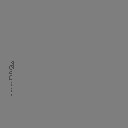
\includegraphics{diff_1}
        \caption{Отличающиеся от исходного пиксели} 
    \end{minipage}
  \end{figure}
  
  \begin{figure}[H]
    \centering
    \begin{minipage}[t]{0.4\textwidth}
        \centering
        
\includegraphics{stego_2}
        \caption{Изображение, со встроенным текстом песни "Yesterday" Beatles}
    \end{minipage}
    \hfill
    \begin{minipage}[t]{0.4\textwidth}
        \centering
        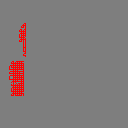
\includegraphics{diff_2}
        \caption{Отличающиеся от исходного пиксели} 
    \end{minipage}
  \end{figure}
  
  \begin{figure}[H]
    \centering
    \begin{minipage}[t]{0.4\textwidth}
        \centering
        
\includegraphics{stego_3}
        \caption{Изображение, со встроенным текстом (частью) книги Айзека Азимова}
    \end{minipage}
    \hfill
    \begin{minipage}[t]{0.4\textwidth}
        \centering
        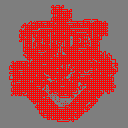
\includegraphics{diff_3}
        \caption{Отличающиеся от исходного пиксели} 
    \end{minipage}
  \end{figure}

  Стоит отметить, что в моей реализации изменяется только красный канал изображения.
  Если производить изменение по остальным (минимум зеленый и синий), то можно
  в 3 раза уменьшить зону отличающихся пикселей.

  Также стоит отметить, что по этим примерам видно, что изображения,
  обладающие малым количество отличий (большие зоны одинаковых блоков)
  меньше подходят для сокрытия в них данных.

  \subsection{Гистограммы изображений}

  Рассмотрим гистограммы исходного (уже интерполированного) и полученных
  в ходе стеганографии изображений:

  \begin{figure}[H]
    \centering
    \begin{minipage}[t]{0.4\textwidth}
        \centering
        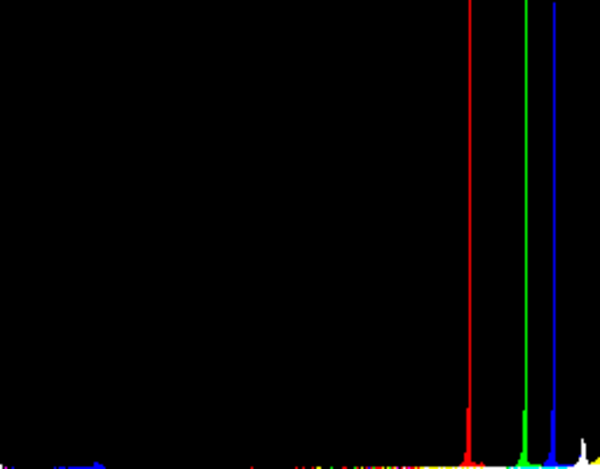
\includegraphics[width=0.8\textwidth]{hist}
        \caption{Исходное изображение}
    \end{minipage}
    \hfill
    \begin{minipage}[t]{0.4\textwidth}
        \centering
        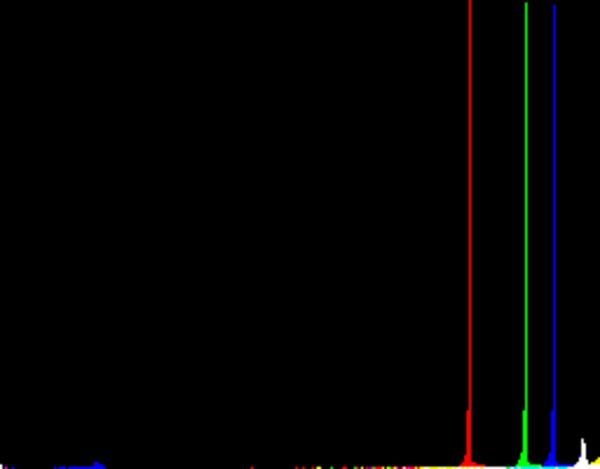
\includegraphics[width=0.8\textwidth]{hist_1}
        \caption{Небольшие изменения} 
    \end{minipage}
  \end{figure}

  \begin{figure}[H]
    \centering
    \begin{minipage}[t]{0.4\textwidth}
        \centering
        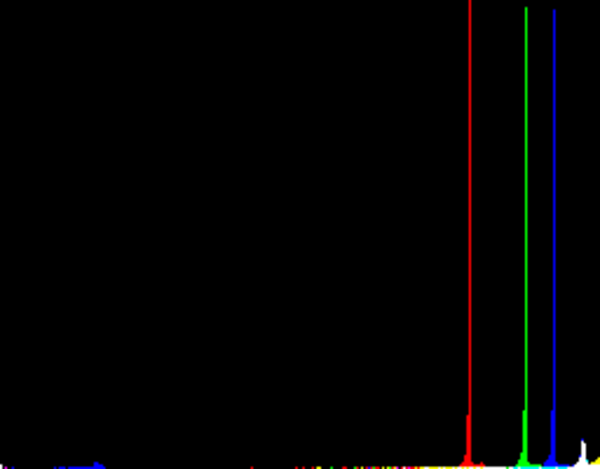
\includegraphics[width=0.8\textwidth]{hist_2}
        \caption{Средние изменения}
    \end{minipage}
    \hfill
    \begin{minipage}[t]{0.4\textwidth}
        \centering
        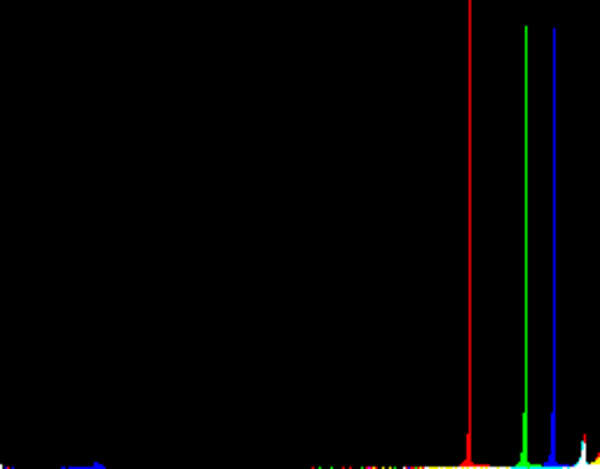
\includegraphics[width=0.8\textwidth]{hist_3}
        \caption{Большие изменения} 
    \end{minipage}
  \end{figure}

  Данные гистограммы как раз и показывают, что количество красного, по сравнению
  с остальными цветами, выросло, что соответствует моей реализации данного алгоритма.

  Чтобы уменьшить эти различия можно производить запись сообщения не только
  по красному каналу, или иногда заменять операцию сложения на операцию вычитания,
  что при определенных данных позволит скомпенсировать этот рост.

  \subsection{Дополнительные эксперименты}

  \subsubsection{Изменения размера изображения - масштабирование}

  Масштабирование приводит к повторной интерполяции сообщения, однако здесь
  коэффициент увеличения сторон изображения может не оказаться равным четко 2,
  что сделает получение сокрытой информации практически невозможным.

  Если же картинка увеличиться в $4^n, n \in \mathbb{N}$ раз, то при таком же примитивном,
  как и в текущей реализации, алгоритмом интерполяции можно, зная коэффициент увеличения,
  поменять алгоритм таким образом, чтобы можно было вытащить исходный текст без потерь,
  однако если увеличение будет происходить таким образом, что исходыне пиксели не будут
  полностью сохранены, то восстановить сообщение опять так не удастся.

  \subsubsection{Изменение размера изображения - кадрирование}

  Кадрирование (обрезка) изображения не так сильно влияет на содержание.
  Если будет удалена та часть картинки, в которой нет информации (отмечены серым),
  то восстановление пройдет успешно без каких либо потерь.

  Если же красная зона будет задета, то часть информации пропадет безвозратно.
  Стоит отметить, что в зависимости от реализации алгоритма, потеря нижней
  половины изображения может быть значетельнее потери правой половины.
  Это происходит по причине того, что сохранение бит исходного сообщения
  может производиться в любом порядке, передвигаясь по пикселям (сверху-вниза,
  справа-налево, зиг-загом и т.п.).

  \subsubsection{Поворот изображения}

  Поворот на любое число градусов,
  точно приведет к невозможности считать сохраненные в изображении данные.
  Однако если вручную повернуть изображение обратно, то сообщение снова станет возможно вернуть.

  Повороты на 90 и 180 градусов наиболее безопасны для сохранности данных,
  так как при повороте на такое число градусов координаты каждого пикселя
  обределяются со 100-процентной точностью, в других случаях что-то может съехать
  и затруднить получение информации.

  \subsubsection{Затемнение и осветвление}

  В зависимости от типа такой операции - относительная или абсолютная, сохранность
  данных различна. При относительном затемнении или осветвлении меняется
  абсолютная разность между значениями пикселей, что делает невозможным
  считывание данных.

  Однако если значение каждого пикселя будет увеличено на какое-то константное значение,
  то в общем случае разница между соседними пикселями останется прежней и данные
  можно будет восстановить.

  \subsubsection{JPEG сжатие}

  Данный алгоритм сжатия нацелен на уменьшение памяти, задействованной
  для хранения одинаковых блоков изображения, а как видно по областям отличающихся
  от исходного изображения пикселей, именно такие зоны не используются
  при JPEG сжатии.

  То есть конвертация из PNG в JPEG потенциально не приведет к потере данных,
  однако что-то все таки может потеряться.

  \newpage
  \section{Вывод}

  Стеганографический метод \textbf{NMI} отлично справляется с встраиваение сообщения
  в изображение контейнер, однако в 4 раза увеличивает его размер, что может
  посодействовать раскрытию факта передачи информации.

  Сам алгоритм показал высокую устойчивость к некоторым видам кадрирования и
  \textit{JPEG} сжатия, однако не прошел проверку масштабированием и поворотом.
  Операции осветвления и затемнения в обычном случае также повредят данные.

  Алгоритм прост в реализации, не требует большой вычислительной мощности.
  Эффективность метода сильно зависит от того, какие цветовые каналы (их количество в частности)
  учавствуют в сохранении информации, а устойчивость к изменениям от порядка,
  в котором пиксели исходного
  изображения перебираются в процессе встраивания изображения.

  Тажке важно, что данный метод позволяет получить достаточну большую плотность
  записи информации.

\end{document}
